%This file will be included in the ThesisMain Document as the experimentation
%section.

%Author: James Kelly
%Last Modified: 11-12-08

\begin{center}
\section{Discussion and Results}
\end{center}

The fundamental motivation for this experimentation was first and foremost to quantify the thermal sink capacity of a bulk aggregate. Additionally, results should demonstrate that a mass of such material can and will remove a measurable amount of thermal energy from a thermally charged flow. Any result short of this hypothesis would effectively render the implementation of aggregate material as a solution to thermally charged stormwater discharge. Infact, some material comes close to being thermally inert with respect to removing adequate amounts of thermal energy from a hydraulic flow. However, most material has demonstated to varying levels an ability to thermally sink a thermall charged flow.
 
It is especially noteworthy in the case of most of the tested materials, given the relatively small thermal heat capacity and thermal conductivities, that the quantity and rates of heat were observed. The experiment was actually contrived on an ounce of suspicion that the materials were stated to have thermal sinking effects primarily out of convienience. Furthermore, some samples offer significant potential to relieve thermal duress under flow in severe scenarios, if implemented properly. It is therefore the goal of this discussion to consider the data and provide a foundation for further research and insight into using non-consolidated materials - of any form - to thermally sink a hydraulic discharge.

\subsection{Characterizing the Thermal Behavior of Aggregates}

Several metrics are used in the performance analyses and ranking of the test materials. Bearing in mind that some of the materials were included in the experimentation strictly to diversify experimental results, several general conclusions can be stated with regard to completely practical materials based on the observed patterns. This section discusses these metrics and explains their role in evaluating a non-consolidated material for thermal sink performance.

Specific intrinsic parameters were identified and used to direct experimentation. Additionally, several environmental variables were also identified and used likewise. The choice of these parameters was based on the expectation that a respective variation would have a measurable effect on the thermal sink capacity of the sample aggregate. Several of these parameters were not directly measured or otherwise included in the current analysis primarily because they exceeded the intended scope of the experiment and available resources, yet based on theoretical renderings may play an important role in a materials thermal response. Some of these parameters include surface porosity, fineness modulus, isotropy, Mohs hardness and cobble geometry. For the purposes of this discussion, such parameters have been ruled as having only peripheral effects compared more dominant parameters as cobble size, bulk density and material, and are consequently not part of this analysis. 

\paragraph{Interpreting the Normalized Cumulative Thermal Sink Function}
In graphically comparing different materials' trials with one another, the Normalized Cumulative Sink Function (NCSF) (Eq \ref{NSCF}) was scaled by the measured heat capacity of the respective trial to yield a function with dimensions J/K/K. This is a function that graphically illustrates the rate at which energy was exchanged with an amplitude that is analogous to the net energy exchanged between water and aggregate. 
\begin{equation}\label{SNCSF}
 SNCSF(t)\;=\;\frac{\delta T(t)[TB]}{\sum_{t=0}^{t_{+Q}}\delta T(t)[TB]}c_{R}
\end{equation}
The primary purpose of creating a SNCSF plot is to rank or compare different aggregate trials. It is a way to visualize and compare thermal sink performance amongst other aggregate families. Plots of the actual energy exchanged are listed in Appendix C, series 2. Below is a SNCSF plot of all medium flows in Figure (\ref{med1}). This plot demonstrates the dominance of material over cobble size, noting how both SB1 (steel balls) and GB1 (glass balls) are 1`` in diameter with nearly identical characteristic radii. Additionally, noting how the aggregate materials have similar specific heats compared to SB1 and GB1, the most variance is a result of cobble size. 

\begin{figure}
 \label{med1}
 \centering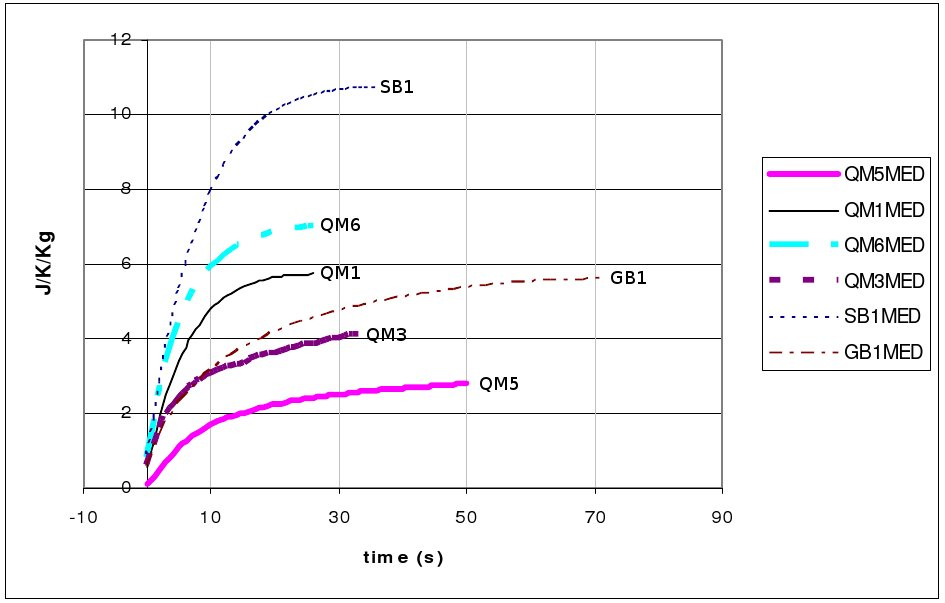
\includegraphics[scale=0.6]{med1.JPG}
 \caption{Scaled, Normalized Cumulative Sink Function from Medium Rate Trials: Each trial is comparable in both a rate and quantity of thermal energy transfer.}
\end{figure}

In Figure (\ref{med1}) two samples, QM.3 and QM5 offer thermal sink performances less than the glass balls. Each of these samples represent the extreme cobble sizes used in the experiments at 0.375'' and 5``, respectively. Noting how the mid-range cobble sizes offer both faster sink rates and total energy transferred during the trial, Figure (\ref{opt1}) demonstrates that infact there is an optimal cobble size for a given set of flow conditions. Note that this plot includes a maximal SNSCF value, so that this is actually expressing the total amount of energy that was transferred for a normalized temperature difference. Two different flows are depicted - a medium and a low flow rate, for comparison. The flow rate seems to be a secondary parameter that stands to increase or decrease the amplitude of the curve while the cobble size will shift the peak of the bell curve left or right. 

\begin{figure}
 \label{opt1}
\centering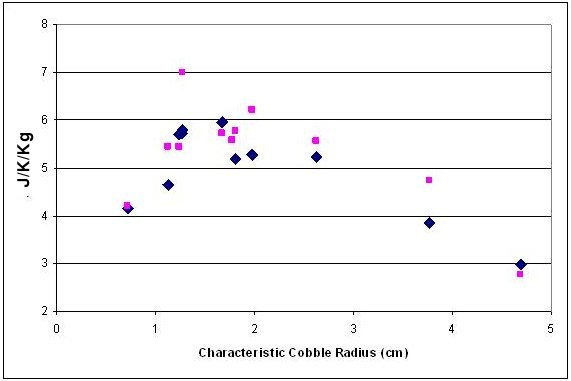
\includegraphics[scale=0.6]{opt2.JPG}
 \caption{SNCSF (J/K/K) versus cobble size demonstrates an optimal cobble size for certain flow conditions. A low flow rate is represented by the diamond symbols, and a medium flow rate is represented by the squares.}
\end{figure}

In studying this trend, the data indicates that as the flow rate increases, the optimal cobble size for thermal sink response should decrease slightly. This is intuitive, knowing that the larger cobbles possess a slower thermal response due to their bulk, and a lower flow can accomodate this best. A higher flow rate - and in turn a higher thermal wattage imparted on the aggregate -  will demand a faster thermal response that a smaller cobble could provide. There are however, flow considerations to bear in mind as well, noting that a decrease in cobble size restricts flow, so in turn there is an optimization boundry. 

Hybred aggregates warrant testing based on these results. It is conceivable that an aggregate of two or more different cobble sizes could offer both flow and thermal sink capacity with some compromise in total bulk. A preliminary analysis of a thermal sink capacity of such a material could be formulated from the current data. However, flow mechanics, the packing ratio and thermal contact parameters will naturally be different with hybred aggregate, and so the exact results are not directly predictable from the current data.

\paragraph{Thermal Conductivity and Diffusivity as Performance Indicators}
Thermal conductivity is an intrinsic characteristic directly related to the material of the aggregate. It simply conveys the rate at which heat is transferred through the material, and it is the usual proportionality constant in modeling thermal energy transfers with the heat equation. Thermal conductivity, as discussed in the experimentation section, is calculated from the data sets and then used to arrive at the thermal diffusivity. A high specific heat, sufficiently large cobble size and high thermal conductivity will help ensure that the aggregate can afford to remove more heat per unit time. All three of these parameters must work together to ensure that a particular sample can remove a significant amount of heat in an adequate period of time. Steel is tested as the ''ideal'' aggregate, as it has an exceptionally high thermal conductivity and specific heat and it acts to quickly remove large amounts of thermal energy. Glass has a very high specific heat -over twice that of the 1018 mild steel used- but it has poor conductivity, and the characteristic response is a long, steady sink. 

Thermal diffusivity is a quantitative measure for a particular mass's ability to respond to a thermal change in its environment. The lower the thermal diffusivity, the less thermal response per unit mass the sample will have. Diffusivity was computed in an attempt to arrive at some bulk unitary index with which to rate an aggregate, independent of flow. It is computed using bulk density and of course bulk temperature differentials, and so it should reflect the response of the entire aggregate mass as a whole. This is said with the assumption that a mass of aggregate will behave differently under duress when compared to a single cobble or material isolate.

\subsection{Recommendations for Thermal Buffering of Watersheds}




\subsection{Recommendations for Research Expansion}



